\documentclass[12pt]{../../../notes}
\usepackage{silence}
\WarningFilter{latex}{Reference}
\graphicspath{{../../img/}}

\begin{document}

\paragraph{Матрицы, основные определения}
\begin{defn}[Матрицы над $K$]\label{defn:matrices}
  Пусть $K$"--- поле, $m,n\in \N$. Тогда
  \[
    M_{m,n}(K) = 
    \left\{
      A 
    \,\middle|\,
      A  = 
      \begin{pmatrix}
        a_{11} & a_{12} & \cdots & a_{1n} \\
        a_{11} & a_{12} & \cdots & a_{1n} \\
        \vdots & \vdots & \ddots & \vdots \\
        a_{m1} & a_{m2} & \cdots & a_{mb}
      \end{pmatrix},\;
      a_{ij} \in K
    \right\}
  \]
\end{defn}

\begin{defn}[Сложение матриц]\label{defn:matradd}
  $A_{mn} + B_{mn}:$
  \[
    (a+b)_{ij} = a_{ij} + b_{ij}
  \]
\end{defn}

\begin{defn}[Умножение матриц]\label{defn:matrmul}
  $A_{mn}\cdot B_{nk}:$
  \[
    (ab)_{ij} = \sum_{\ell=1}^n a_{i\ell}\cdot b_{\ell j}
  \]
\end{defn}

\paragraph{Кольцо квадратных матриц}
Обозначается $M_n(K)$

\noindent Ноль:
\[
  Z_n = 
  \begin{pmatrix}
    0      & 0      & \cdots & 0 \\
    0      & 0      & \cdots & 0 \\
    \vdots & \vdots & \ddots & \vdots \\
    0      & 0      & \cdots & 0 \\
  \end{pmatrix}
\]
Единица:
\[
  E_n = 
  \begin{pmatrix}
    1      & 0      & \cdots & 0 \\
    0      & 1      & \cdots & 0 \\
    \vdots & \vdots & \ddots & \vdots \\
    0      & 0      & \cdots & 1 \\
  \end{pmatrix}
\]
\parrange{2}{Определитель}
\begin{defn}\label{defn:determinant}
  Пусть $A\in M_n(K)$
  \[
    \det A = \sum_{\sigma \in S_n} (-1)^{I(\sigma)} \cdot a_{1\sigma(1)} \dotsm a_{n\sigma(n)}
  \]
\end{defn}
\begin{defn}\label{defn:determrows}
  Если обозначать строки $A_1, \dotsc , A_n$, а столбцы $A^{(1)}, \dotsc , A^{(n)}$,
  то можно ввести ещё такую функцию:
  \[
    \det (A_1, \dotsc , A_n) = \det (A^{(1)}, \dotsc , A^{(n)}) := \det A
  \]
\end{defn}

\begin{defn}[Элементарные преобразования]\label{defn:elemtranf}
  \noindent\newline\par
  \begin{enumerate}[I]
    \item\label{it:transfchng}   \makebox[8em][l]{$A_i \leftrightarrows A_j$} 
      $A^{(i)} \leftrightarrows A^{(j)}$     
    \item\label{it:transfaddmul} \makebox[8em][l]{$A_i := A_i + \lambda A_j$} 
      $A^{(i)} := A^{(i)} + \lambda A^{(j)}$ 
    \item\label{it:transfmul}    \makebox[8em][l]{$A_i := \lambda A_i$}       
      $A^{(i)} := \lambda A^{(i)}$           
  \end{enumerate}
\end{defn}
\begin{defn}[Транспонированная матрица]\label{defn:transpose}
  \[
    A^T \colon (a^T)_{ij} = (a)_{ij}
  \]
\end{defn}

\subparagraph{Свойства}
\begin{enumerate}
  \item Определитель (в описанном в~\ref{defn:determrows} смысле) полилинеен и кососимметричен по
    строкам и столбцам.
  \item Если 2 строчки или столбца одинаковые, то определитель равен 0
  \item Элементарные преобразования влияют на определитель следующим образом:\par
    \begin{tabular}{c|r}
      I   & $(-1)\det A$ \\
      II  & $\det A$     \\
      III & $\lambda \det A$
    \end{tabular}
  \item $\det A^T = \det A$
\end{enumerate}


\paragraph{Теорема Лапласа}
\begin{defn}[Минор]\label{defn:minor}
  Пусть $A\in M_n(K)$, а $k\in \N$. Тогда определитель подматрицы, собранной из $k$ строк и $k$
  столбцов называется \emph{минором} порядка $k$.
  \[
    \Delta = 
    \begin{vmatrix}
      a_{i_1j_1} & \cdots & a_{i_1j_k} \\
      \vdots & \ddots & \vdots \\
      a_{i_kj_1} & \cdots & a_{i_kj_k} 
    \end{vmatrix}
  \]
  $\Delta'$~--- дополнительный минор"--- всё, что осталось.
  Его ещё иногда (когда минор"--- один элемент) обозначают как $M_{ij}$
\end{defn}
\begin{defn}[Алгебраическое дополнение]\label{defn:cofactor}
  \[
    A_\Delta = (-1)^{i_1 + \dotsb + i_k + j_1 + \dotsb + j_k} \Delta'
  \]
\end{defn}

\begin{thrm}[Теорема Лапласа]\label{thrm:laplacecofactor}
  Пусть $A\in M_n(K)$, $k\in \N$. Выберем из матрицы $k$ строчек. Тогда
  \[
    \det A = \sum_{\Delta} \Delta \cdot A_\Delta
  \]
  где $\Delta$~--- любой минор, содержащий нужные $k$ строчек.
\end{thrm}
\begin{ittproof}
  Выберем какой-то один минор, $i_k$~--- его строчки, $j_\ell$~--- его столбцы
  \[
    \Delta : 
    \begin{cases}
      i_1, \dotsc , i_k \\
      j_1, \dotsc , j_k
    \end{cases}
  \]
  Теперь отправим все элементы, попавшие в минор, в левый верхний угол.
  Сначала сдвинем все строчки:
  \[
    \begin{cases}
      i_1 \to 1 & (i_1 -1 \text{~сдвигов})\\
      \hdotsfor{2} \\
      i_k \to k & (i_k - k \text{~сдвигов})
    \end{cases}
  \]
  Потом все столбцы
  \[
    \begin{cases}
      j_1 \to 1 & (i_1 - 1 \text{~сдвигов})\\
      \hdotsfor{2} \\
      j_k \to k & (i_k - k \text{~сдвигов})
    \end{cases}
  \]
  В итоге, из свойств элементарных преобразований, получим: 
  \[
    \det B = (-1)^{i_1 - 1 + \dotsb + i_k - k + j_1 - 1 + \dotsb + j_k - k} \det A 
    = (-1)^{i_1  + \dotsb + i_k  + j_1  + \dotsb + j_k } \det A 
  \]
  так как все добавки парные $\Rightarrow$ делится на $2$.

  С другой стороны, $\Delta$ и $\Delta'$ никак не поменялись, так как переставляемые чиселки в
  них не не входят. Также нужно отметить, что $B_\Delta = \Delta'$, по тем же причинам, в
  общем-то.

  Посмотрим, что такое  $\Delta\cdot \Delta'$
  \footnote{Вообще, тут маленькая неточность: здесь фактически 
      \emph{действие} группы перестановок на множестве $\{k+1, \dotsc , n\}$}.
  \begin{align*}
    \Delta \cdot \Delta' 
    &= \Bigg( \sum_{\tau \in S_k} (-1)^{I(\tau)} b_{1\tau(1)} \dotsm
    b_{k\tau(k)} \Bigg) \cdot \Bigg( \sum_{\tau' \in S_{n-k}} (-1)^{I(\tau')} b_{k+1\tau'(k+1)} \dotsm
    b_{n\tau(n)} \Bigg)
  \end{align*}
  Пусть теперь $\sigma = \tau \circ \tau'$. Тогда $I(\sigma) = I(\tau)+I(\tau')$ по свойствам
  перестановок, а $\sigma$ фактически разбивается на 2 независимых: $\tau$ и $\tau'$.
  В итоге
  \[
    \Delta \cdot \Delta' 
    = \sum_{\sigma\in S_n} (-1)^{I(\sigma)} b_{1\sigma(1)} \dotsm b_{n\sigma(n)}
  \]
  А это вообще-то правильный кусок определителя $B$. 
  Поймём, что это за кусок определителя $A$.
  Числа-то те же самые. А вот на вопрос со знаком мы уже по сути ответили, когда рассуждали про 
  определитель. Слагаемые точно не смешиваются, так как все перестановки"--- биекции, 
  так что каждое слагаемое просто умножается на $(-1)^{\cdots}$. Мы же ещё когда доказывали свойства определителя,
  выяснили, что там каждое слагаемое меняет знак так же, как и определитель.
  Так что 
  \begin{align*}
    \Delta \cdot \Delta' &= (-1)^{i_1  + \dotsb + i_k  + j_1  + \dotsb + j_k } 
    \sum_{\sigma'} a_{1\sigma'(1)} \dotsm a_{n\sigma'(n)} \\
    A_{\Delta} &= (-1)^{i_1  + \dotsb + i_k  + j_1  + \dotsb + j_k } \Delta'  \\
    \Delta \cdot A_{\Delta} &= \sum_{\sigma'} a_{1\sigma'(1)} \dotsm a_{n\sigma'(n)}
  \end{align*}
  где у $\sigma'$ уже другие независимые циклы: ${i_1, \dotsc , i_k\choose j_1, \dotsc , j_k }$ 
  и всё остальное.
\end{ittproof}
\begin{imp}
  \[
    \det A = a_{i1} A_{i1} + \dotsb + a_{in} A_{in} 
  \]
\end{imp}
\begin{imp}
  \[
    a_{j1} A_{i1} + \dotsb + a_{jn} A_{in} = 0
  \]
\end{imp}
\begin{itlproof}
  Приравняем $i$ строчку к $j$-ой, получим матрицу $B$. Тогда
  \[
    a_{j1} A_{i1} + \dotsb + a_{jn} A_{in} = b_{i1} B_{i1} + \dotsb + b_{jn} B_{in} = \det B = 0
  \]
  Так как определитель $B$ очевидно равен 0
\end{itlproof}

\paragraph{Ступенчатая матрица}

\begin{defn}\label{defn:stairsmtx}
  $A$ = \raisebox{-0.45\height}{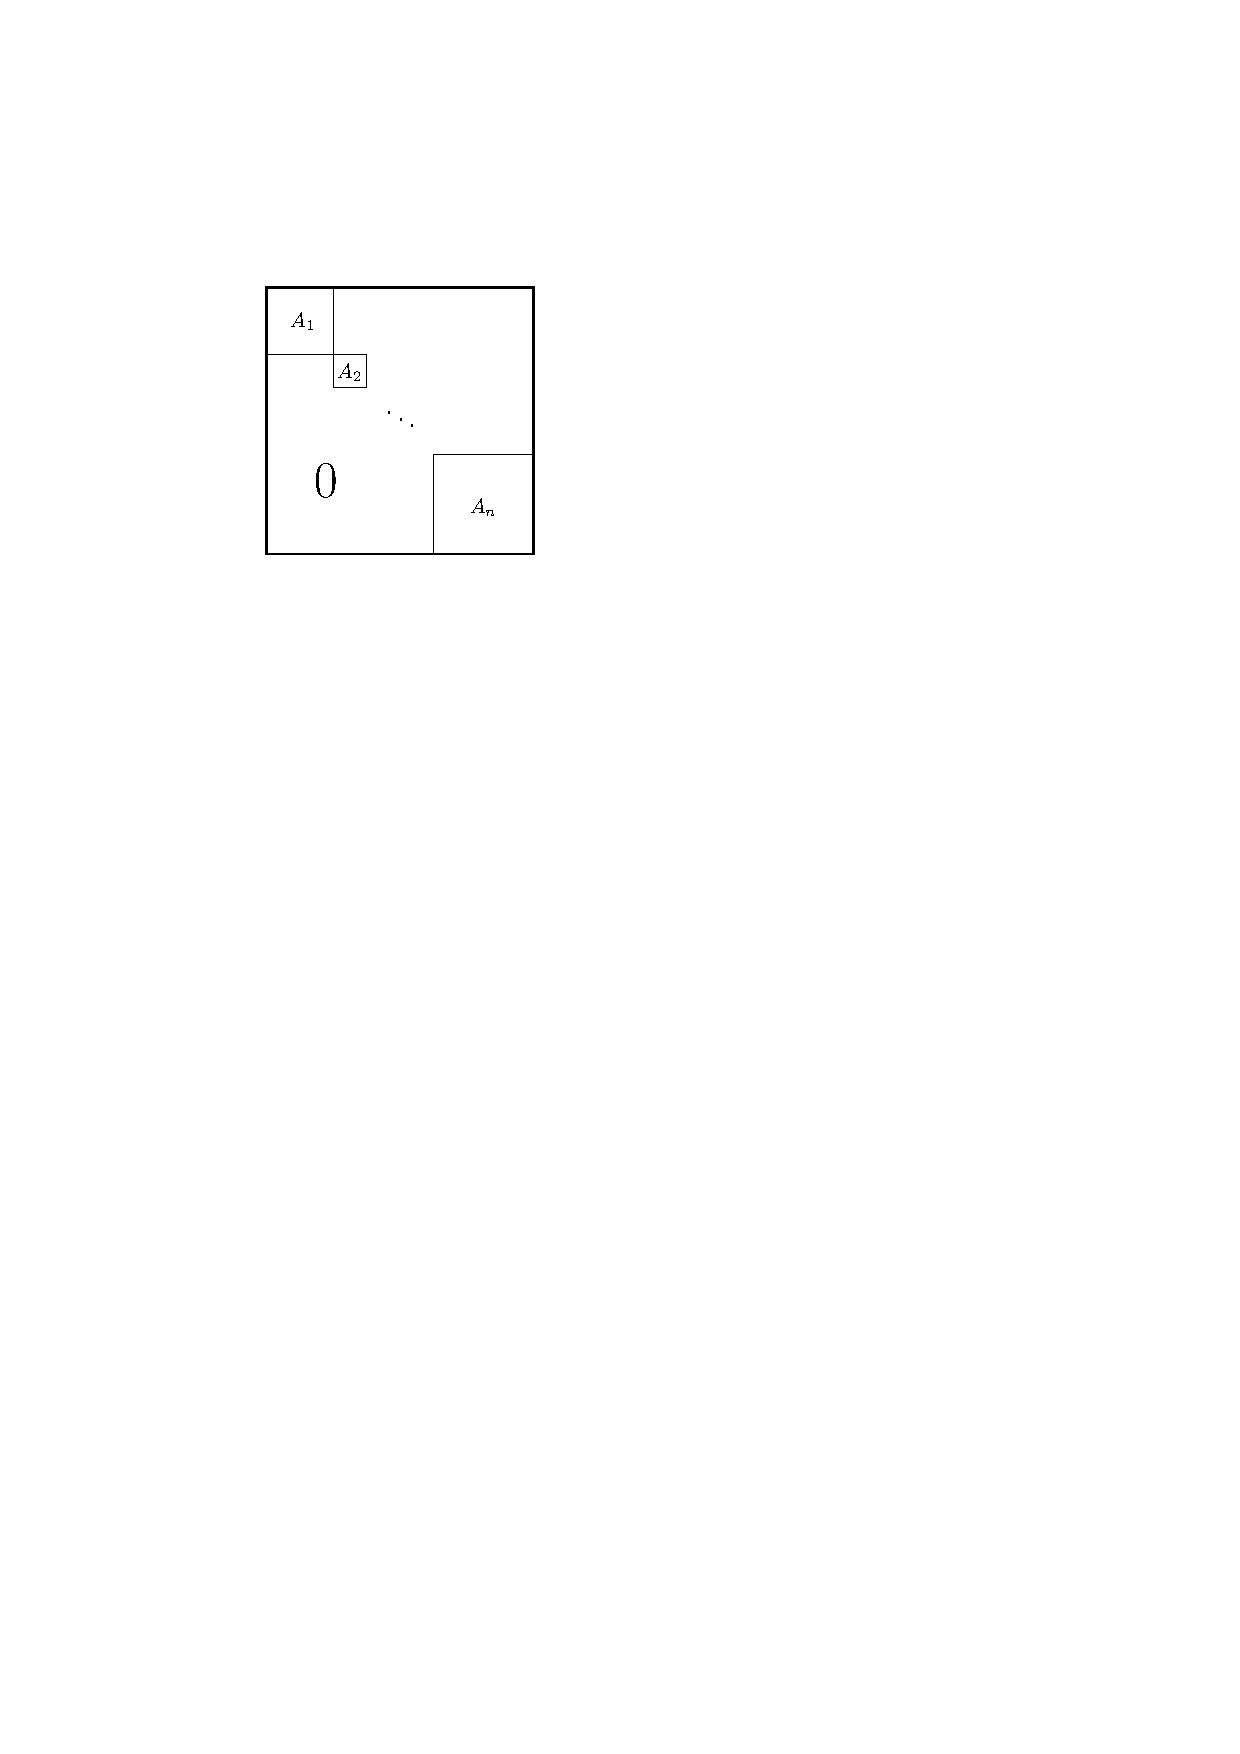
\includegraphics[scale=0.6]{stairsmtx}}~--- ступенчатая 
  матрица.\footnote{некоторые называют такую матрицу квазитреугольной, а ступенчатую~--- трапецевидной}
\end{defn}
\begin{thrm}[Определитель ступенчатой матрицы]\label{thrm:stairsdet}
  \[
    \det A = \det A_1 \dotsm \det A_n
  \]
\end{thrm}
\begin{ittproof}
  По индукции через теорему Лапласа~\ref{thrm:laplacecofactor}
\end{ittproof}

\paragraph{Определитель произведения матриц}
\begin{thrm}\label{thrm:detmult}
  Пусть $A,B \in M_n(K)$. Тогда
  \[
    \det (AB)  = \det A \cdot \det B
  \]
\end{thrm}
\begin{ittproof}
  Докажем, что такие матрицы имеют одинаковый определитель:
  \[
    C = 
    \left(
    \begin{array}[h]{c|c}
      A    & 0 \\
      \hline 
      -E_n & B
    \end{array}
    \right) \quad \text{и} \quad 
    D = 
    \left(
    \begin{array}[h]{c|c}
      AB    & A \\
      \hline 
      0 & -E_n
    \end{array}
    \right)
  \]
  Теперь сделаем из куска с $B$ $Z_n$. 
  \[
    D'^{(n+j)} := C^{(n+j)} + b_{1j} C^{(1)} + \dotsb + b_{nj} C^{(n)}
  \]
  Внизу получатся нули, а вот сверху:
  \[
    d_{i,n+j} = 0 + b_{1j} a_{i1} + \dotsb + b_{nj} a_{in} = (ab)_{ij}
  \]
  Тысяча индексов, это же произведение матриц!
  \[
    D' = \left(
    \begin{array}[h]{c|c}
      A    & AB \\
      \hline 
      -E_n & 0
    \end{array}
    \right) 
  \]
  Мы тут пользовались только преобразованием \ref{it:transfaddmul}, так что определитель не
  поменялся. 

  Теперь переставим половинки матрицы. При этом будет совершено $n$ 
  преобразований~\ref{it:transfchng}. Так что
  \[
    \begin{split}
      \det A \det B & = \det C = \det D' = (-1)^n \det D = (-1)^n \det(-E_n) \det(AB) \\
                    & =  (-1)^{2n} \det(AB) = \det AB
    \end{split}
  \]
\end{ittproof}

\paragraph{Обратимость матриц}

\begin{defn}\label{defn:nonzerodet}
  Пусть $A = M_n(K)$. Тогда $A$~--- невырожденная $\Leftrightarrow$ $\det A \neq 0$
\end{defn}
\begin{defn}[Взаимная матрица]\label{defn:adjointmtx}
  \[
    \widetilde{A} = (a)_{ij}^T
  \]
\end{defn}

\begin{lem}\label{lem:adjointmtx}
  \[
    A\cdot\widetilde A = \det A \cdot E_n
  \]
\end{lem}

\begin{defn}\label{defn:invertmtx}
  Пусть $A = M_n(K)$. Тогда матрица $A^{-1}:$
  \[
    A\cdot A^{-1} = A^{-1} \cdot A = E_n
  \]
  (если существует)
\end{defn}

\begin{imp}
  Если $\det A \neq 0$, то
  \[
    A^{-1} = \frac{1}{\det A} \widetilde{A}
  \]
\end{imp}

\begin{imp}
  А невырождена $\Leftrightarrow$ А"--- обратима. 
\end{imp}

\begin{imp}
  Пусть $A,B \in M_n(K)$. Тогда 
  \[
    AB = E_n \Rightarrow A,B \text{~--- обратимы и } 
    \begin{cases}
      B = A^{-1} \\
      A = B^{-1}
    \end{cases}
  \]
\end{imp}

\parrange{2}{Ранг, строчный и столбцовый}
\begin{defn}[Строчный ранг]\label{defn:rowrank}
  Пусть $A\in M_{m,n}(K)$. Тогда \[
    \rk_s (A) = \dim \langle A_1, \dotsc , A_m \rangle
  \]
\end{defn}

\begin{defn}[Столбцовый ранг]\label{defn:colrank}
  Пусть $A\in M_{m,n}(K)$. Тогда \[
    \rk^{(s)} (A) = \dim \langle A^{(1)}, \dotsc , A^{(m)} \rangle
  \]
\end{defn}

\begin{lem}\label{lem:rowranktransf}
  Строчный ранг сохраняется при элементарных преобразованиях строк.
\end{lem}
\begin{itlproof}
  Пусть $B_1, \dotsc , B_m$ получены из $A_1, \dotsc , A_m$ элементарными преобразованиями строк.
  Эти преобразования"--- линейные.\footnote{Вообще, конечно, так нехорошо. Линейные отображения 
  ещё не ввели, так что надо каждое преобразование проверять}.
  Так что линейная оболочка никак не изменится. 
  \[
    \langle A_1, \dotsc , A_m\rangle = \langle B_1, \dotsc , B_m\rangle
  \]
  А значит, и ранги совпадают.
\end{itlproof}
Транспонирование даст аналогичное рассуждение для столбцов

\begin{lem}\label{lem:colranktransf}
  Столбцовый ранг сохраняется при элементарных преобразованиях строк.
\end{lem}
\begin{itlproof}
  Пусть $\rk^{(s)} (A) = r$.
  Будем по одному убирать из линейной оболочки столбцов линейно выражающиеся векторы
  \[
    \langle A^{(1)}, \dotsc , A^{(n)}\rangle \rightsquigarrow 
    \langle A^{(i_1)}, \dotsc , A^{(i_r)}\rangle
  \]
  Пусть после линейных преобразований образы этих векторов стали линейно зависимы, 
  $A \rightsquigarrow B$. Перепишем:
  \begin{align*}
    \beta_1 B^{(i_1)}+ \dotsb + \beta_n B^{(i_r)} = 0 
    \Leftrightarrow
    \begin{cases}
      b_{1i_1} \beta_1 + \dotsb + b_{1i_r} \beta_n = 0\\
      \hdotsfor{1} \\
      b_{mi_1} \beta_1 + \dotsb + b_{mi_r} \beta_n = 0
    \end{cases} \quad (\exists\, \beta_i \neq 0)
  \end{align*}
  Проведём все преобразования в обратную сторону. Тогда, $\{\beta_i\}$ тоже останутся решениями
  такой системы уравнений, так как все преобразования не изменят решений.
  А тогда и $\{A^{i_k}\}$~--- линейно зависимы(?!?).

  Таким образом, $\rk^{(s)} B \geqslant \rk^{(s)} A$. Теперь можно поменять всюду $A$ и $B$ местами.
  В силу обратимости элементарных преобразований рассуждение не изменится. 
  Так что $\rk^{(s)} A \geqslant \rk^{(s)} B$. А тогда $\rk^{(s)} A = \rk^{(s)} B$.
\end{itlproof}
Транспонирование даст аналогичное рассуждение для строчек

\paragraph{Ранг матрицы}


\begin{thrm}\label{thrm:rowrk=colrk}
  Строчный и столбцовый ранг совпадают
\end{thrm}
\begin{ittproof}
  Тут рисовать надо, а я пока не умею это делать быстро..$\ddot{\frown}$
  Будем приводить матрицу к такому виду:
  \[
    \left(
    \begin{array}{c|c}
      E_r & 0 \\ \hline
      0   & 0
    \end{array}
    \right)
  \]
  \begin{enumerate}
    \item Найдём ненулевой элемент, поставим в $1,1$ преобразованием~\ref{it:transfchng}
    \item С помощью преобразования~\ref{it:transfaddmul} для строк сделаем нулевым весь первый
      столбец, кроме $1,1$. 
    \item Теперь с помощью такого же преобразования для столбцов сделаем первую строку нулевой,
      кроме первого элемента.
    \item Поделим первую строку на первый элемент
    \item Выкинем первую строку и первый столбец, повторив всё для остальной матрицы
  \end{enumerate}
  Даже такие издевательства над бедной матрицей не изменят оба ранга.
  А в преобразованной они очевидно равны
\end{ittproof}

\begin{defn}[Ранг матрицы]\label{defn:mtxrank}
  \[
    \rk A := \rk_s (A) = \rk^{(s)} A
  \]
\end{defn}

\paragraph{Ранги и миноры}
\begin{thrm}\label{thrm:rkminor}
  Ранг матрицы"--- наибольший порядок\footnote{размер подматрицы соответствующей минору, проще
  говоря.} её ненулевого минора.
\end{thrm}
\begin{ittproof}
  Пусть $\rk A = r$. Тогда строки всех миноров порядка $s > r$ линейно зависимы. А значит, можно 
  элементарными преобразованиями получить строку нулей. Значит, наибольший порядок минора
  $\leqslant r$. 

  Докажем, что минор порядка $r$ подходит. Выберем $r$ линейно независимых строк и из них вытащим
  подматрицу. Убедимся, что её определитель ненулевой.
  Можно преобразовать её всё тем же алгоритмом, что был описан в теореме~\ref{thrm:rkminor},
  разве что делить первую строку чтобы получить 1 не будем.
  Если где-то появится нулевая строка, значит строки были линейно зависимы. А матрица ещё была
  квадратной. Так что получится матрица диагонального вида. Определитель посчитать нетрудно, он
  получается ненулевой.
\end{ittproof}

\paragraph{Матричная запись СЛУ и решения такой системы}
\begin{defn}\label{defn:matrslineq}
Рассмотрим какую-то систему линейных уравнений

\begin{equation}
  \begin{cases}
    a_{11} x_1 + \dotsb +a_{1n} x_n = b_1\\
    \hdotsfor{1} \\
    a_{m1} x_1 + \dotsb +a_{mn} x_n = b_1
  \end{cases}
  \label{eq:sleq}
\end{equation}

Можно записать её в таком виде:
\[
  A\cdot X = B
\]
где $A$~--- матрица системы, $X$~--- столбец неизвестных, $B$~--- столбец решений, умножение
матричное.

Однородную систему уравнений можно записать как $A\cdot X = 0$
\begin{equation}
  \begin{cases}
    a_{11} x_1 + \dotsb +a_{1n} x_n = 0\\
    \hdotsfor{1} \\
    a_{m1} x_1 + \dotsb +a_{mn} x_n = 0
  \end{cases}
  \label{eq:hsleq}
\end{equation}

\end{defn}

\begin{thrm}\label{thrm:homsystsolspc}
  Решение однородной системы линейных уравнений"--- подпространство $K^n$, причём размерность
  пространства решений"--- количество главных (основных, базисных) переменных.
\end{thrm}
\begin{ittproof}
  Приведём матрицу к ступенчатому как это определено тут~\cite[стр.~50]{Vinberg} виду. Нигде это нормально не 
  определялось, но и так очевидно что это и как получается. Я рисуночек хотел вставить, но не
  успею.
  
  Тогда главные переменные"--- те, что которые соответствуют числа, \emph{не} стоящие на краях 
  <<ступенек>>. Пусть $i_1, \dotsc , i_k$~--- их номера. Тогда рассмотрим $\{e_j\}$, такие, что
  \[
    e_j = 
    \begin{pmatrix}
      \vdots \\
      0 \\
      \vdots \\
      1 \\
      \vdots \\
      0\\
      \vdots
    \end{pmatrix}
    \begin{matrix}
      \vdots \\
      i_1 \\
      \vdots \\
      i_j \\
      \vdots \\
      i_k\\
      \vdots
    \end{matrix}
  \]
  причём остальные чиселки в этих векторах выбираются с тем условием, что $A e_j = 0$.

  Все $e_j$ разные, так что система линейно независима. Теперь докажем, что все решения
  порождаются такой системой векторов. 

  Пусть $x$~--- столбец решений. Соберём
  \[
    x^* = x_{i_1} e_i + \dotsb +x_{i_k} e_k 
  \]
  Если подумать до конца своих дней, то можно осознать, что
  \[
    \begin{cases}
      A x = 0 \\
      A x^* = 0
    \end{cases} \Rightarrow x-x*\text{~--- решение}.
  \]
  Оказалось, что думать до конца своих дней не нужно, ведь векторы $e_j$ определены так, что  
  $Ax^* = 0$. 
  
  Итак, мы выяснили, что $x-x^*$ решение. Но у этого вектора на всех позициях, соответствующих
  главным переменным стоят нули. А раз он решение, то и на всех остальных местах нули.
  (ну, иначе $1\cdot x_1 \neq 0$, например). Тогда $x = x^*$.

  Чудно, мы получили что можем таким хитрым базисом породить все решения. Докажем, что
  решения"--- подпространство.
  
  Пусть $x^1, x^2$~--- решения. Тогда
  \[
    A(\lambda x^{(1)} + \mu x^{(2)}) = \lambda A x^{(1)} + \mu A x^{(2)} = \lambda 0 + \mu 0 = 0
  \]
  Тогда по лемме~\ref{lem:linspsign} оно подпространство. А выбранные векторы $e_j$~--- базис,
  так как они порождают все решения и линейно независимы.
\end{ittproof}  

\begin{defn}\label{defn:fundsol}
  Базис пространства решений ОСЛУ~--- фундаментальная система решений.
\end{defn}

\begin{thrm}\label{thrm:dimsolnslq}
  Пусть~\eqref{eq:hsleq}~--- однородная система линейных уравнений. Тогда размерность
  пространства её решений равна $m - \rk A$, где $m$~--- порядок матрицы.
\end{thrm}
\begin{ittproof}
  Если сделать матрицу ступенчатой с единицами на <<ступеньках>> , то её ранг не изменится. 
  Размерность строк приведённой матрицы~--- это число <<ступенек>>. 
  А последнее равно $m-k$, где $k$~--- число главных переменных.
\end{ittproof}

\begin{thrm}\label{thrm:homtoordlinsys}
  Пусть $V$~--- пространство решений \eqref{eq:hsleq}, $U$~--- множество решений \eqref{eq:sleq},
  $x^0\colon Ax^0 = B$. Тогда $U =  V+ x^0$~--- аффинное подпространство $K^n$ 
\end{thrm}
\begin{ittproof}
  Пусть $x \in V + x^0$. Тогда $x = x'+ x^0$, $x' \in V$.
  \[
    A x = Ax' + Ax^0 = B + 0 = B \Rightarrow x\in U \Rightarrow V + x^0 \subset U
  \]
  С другой стороны, пусть $y \in U$. Тогда 
  \[
    A(y - x^0) = Ay - Ax^0 = 0 \Rightarrow y \in V+x^0 \Rightarrow U \subset V+ x^0 
  \]
\end{ittproof}

\paragraph{Теорема Кронекера-Капелли}

\begin{defn}\label{defn:compsysleq}
  Система уравнений вида $Ax=B$ называется совместной, если она имеет решение.
\end{defn}

\begin{defn}[Расширенная матрица сиситемы]\label{defn:extmtx}
  \[
    (A|B) = 
    \begin{pmatrix}
      a_{11} & \cdots & a_{1n} & b_1 \\
      \hdotsfor{4} \\
      a_{m1} & \cdots & a_{mn} & b_1 
    \end{pmatrix}
  \]
\end{defn}
\begin{thrm}[Кронекера-Капелли]\label{thrm:kronkap}
  СЛУ $Ax =B$ совместна $\Leftrightarrow \rk (A) = \rk (A|B)$
\end{thrm}
\begin{ittproof}
  \begin{description}
    \item[\circlearound{$\Rightarrow$}] 
      \[
        A x = B \Rightarrow A^{(1)} x_1 + \dotsb + A^{(n)} x_n = B
      \]
      Таким образом, $B$ выражается через $A^{(1)}, \dotsc , A^{(n)}$.
      Следовательно,
      \[
        B \in \langle A^{(1)}, \dotsc , A^{(n)}\rangle 
        \Rightarrow 
        \langle A^{(1)}, \dotsc , A^{(n)}\rangle  = \langle A^{(1)}, \dotsc , A^{(n)}, B\rangle 
      \]
      А тогда равны их размерности $\Rightarrow$ равны ранги.
    \item[\circlearound{$\Leftarrow$}] 
      Раз равны ранги, то равны и размерности линейных оболочек столбцов. А раз прибавление
      вектора $B$ не меняет размерности, то он линейно выражается через остальные. Дальше уже
      совсем ясно.
  \end{description}
\end{ittproof}

\paragraph{Матрицы элементарных преобразований}
\begin{enumerate}[I]
  \item $\displaystyle
      E_{ij} = \bordermatrix{
        ~ & ~      & i      & ~      & j      &        \cr
        ~ & E_n    & \vdots & 0      & \vdots & 0      \cr
        i & \cdots & 0      & \cdots & 1      & \cdots \cr
        ~ & 0      & \vdots & E_n    & \vdots & 0      \cr
        j & \cdots & 1      & \cdots & 0      & \cdots \cr
        ~ & 0      & \vdots & 0      & \vdots & E_n    \cr
      }
    $
  \item $\displaystyle
      E_{ij}(\lambda) = \bordermatrix{
        ~ & ~      & j      & ~      & ~      &        \cr
        ~ & E_n    & \vdots & 0      & \vdots & 0      \cr
        ~ & \cdots & 1      & \cdots & 0      & \cdots \cr
        ~ & 0      & \vdots & E_n    & \vdots & 0      \cr
        i & \cdots & \lambda& \cdots & 1      & \cdots \cr
        ~ & 0      & \vdots & 0      & \vdots & E_n    \cr
      }
    $
  \item $\displaystyle
      E_{i}(\lambda) = \bordermatrix{
        ~ & ~      & i       & ~      \cr
        ~ & E_n    & \vdots  & 0      \cr
        i & \cdots & \lambda & \cdots \cr
        ~ & 0      & \vdots  & E_n    \cr
      }
    $
\end{enumerate}
Умножение слева преобразует строки, справа"--- столбцы.

\subparagraph{Поиск обратной матрицы}
Можно привести матрицу, как уже много раз делали, к такому виду
\[
  A \rightsquigarrow 
  \begin{pmatrix}
    E_r & 0 \cr
    0  & 0 \cr
  \end{pmatrix} = M
\]
\begin{enumerate}[1)]
  \item $M \neq E_n \Rightarrow A$ необратима. 
  \item $M = E_n$.
    \begin{align*}
      E_n &= \underbrace{P_\ell \dotsm P_1}_{\mathclap{\text{преобразования строк}}} \cdot  A  \cdot
      \overbrace{Q_1 \dotsm Q_s}^{\mathclap{\text{преобразования столбцов}}} \\
      A &= P_1^{-1} \dotsm P_\ell^{-1} E_n Q_s^{-1} \dotsm Q_1^{-1} \\
      A^{-1} &=  Q_1 \dotsm Q_s P_\ell \dotsm P_1
    \end{align*}
\end{enumerate}
Отсюда кстати проистекает волшебный способ поиска обратной матрицы~--- написать рядом с ней
единичную и преобразованиями строк получить из неё единичную. Тогда там, где была единичная
матрица, получится обратная к $A$.

\end{document}
